\subsection{Perceptron} \label{subs:perceptron}
The perceptron was first developed in 1957 by \textcite{brain_perceptron_nodate}. It is a computational model based on the human brain. The brain is composed of a huge number of computing units, where each unit is called a \textbf{neuron}. A biological neuron receives information (collects charges) from its synapses through chemical mechanisms. Once a certain threshold is passed, the cumulate charges are released (we say the neuron fires). The information is therefore transmitted to other neurons through its synapses.

We can translate this biological neuron into a mathematical form: the perceptron, an artificial neuron. The perceptron has $n_{in}$ inputs $\boldsymbol{x} = \{ x_1, ... x_{n_{in}} \}$, $n_{in}$ weights $\boldsymbol{w}$ and a bias $b$. The perceptron, when receiving an input, performs a weighted sum of the input vector $\boldsymbol{x}$. If the result of the weighted sum is greater than a threshold (controlled by the bias $b$, which can lower or raise it), the perceptron is 'activated' and outputs a non-zero value (1). We can observe this process in figure \ref{fig:perceptron}.
In this case, the mathematical formula described can be written as in equation \eqref{eq:perceptron}, where $h$ is the activation function of the perceptron (see equation \eqref{eq:step}). More details about the activation functions can be found in section \ref{subs:acti}.
%
\begin{equation}
    h ( \boldsymbol{x} | \boldsymbol{w}, b) = h(\sum^{n_{in}}_{i=1} x_i \cdot w_i + b) = h ( \boldsymbol{w}^{T} \cdot \boldsymbol{x} + b)
    \label{eq:perceptron}
\end{equation}
%
\begin{equation}
    h ( \boldsymbol{w}^{T} \cdot \boldsymbol{x} + b) = \begin{cases} 1, & \mbox{if } \boldsymbol{w}^{T} \cdot \boldsymbol{x} + b > 0 \\ 0, & \mbox{Otherwise} \end{cases}
    \label{eq:step}
\end{equation}
%
As the perceptron performs a weighted sum, those can be learned to perform a particular task. However, this model is limited by the functions it can achieve. In section \ref{subs:fcl}, we discover how we can use multiple perceptrons to create a \textbf{fully-connected layer} to learn more complex functions.
%
\begin{figure}
    \centering
    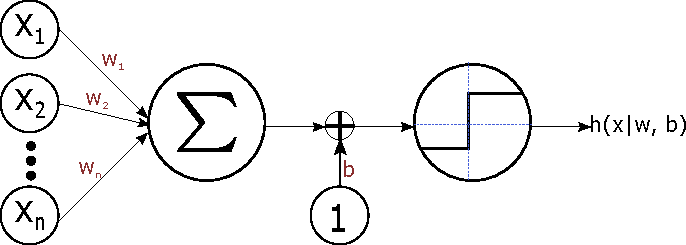
\includegraphics[width=\textwidth]{perceptron.pdf}
    \caption{The Perceptron}
    \label{fig:perceptron}
\end{figure}
